
\section{Personnages}
\lettrine{L}{e} c\oe{}ur des jeux de rôle réside dans la possibilité de créer, améliorer et faire évoluer son propre personnage. Voilà comment ça fonctionne dans {\jedifont Starwars reloaded}. 

\subsection{Races Jouable}
Vous pouvez choisir pour votre personnage n’importe quelle race disponible dans l'univers de Starwars. 

\begin{monsterbox}{Humain}
	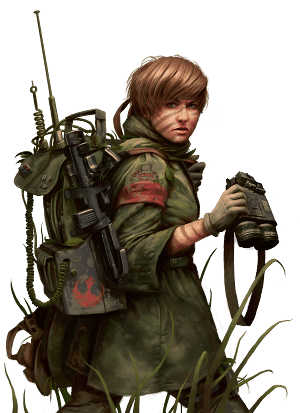
\includegraphics[width=5cm]{img/races/humain.png}
	\hline
	\basics[%
		type = Humain,
		planet = Terre,
		language = Basic
	]
	\hline
	\traits
	\stats
	\hline
	Cette race comprend aussi bien les humains au sens strict (qu’ils soient originaires de Coruscant, de Correlia, de Kuat, de Naboo...) que les humanoïdes dont les caractéristiques physiques, intellectuelles, sociales et culturelles sont suffisamment proches de celles des humains pour qu’il soit possible de les assimiler en termes de jeu. Cela inclut par exemple les iridoniens (zabraks) et les dévaroniens.
\end{monsterbox}

\begin{monsterbox}{Barabel}
	\textit{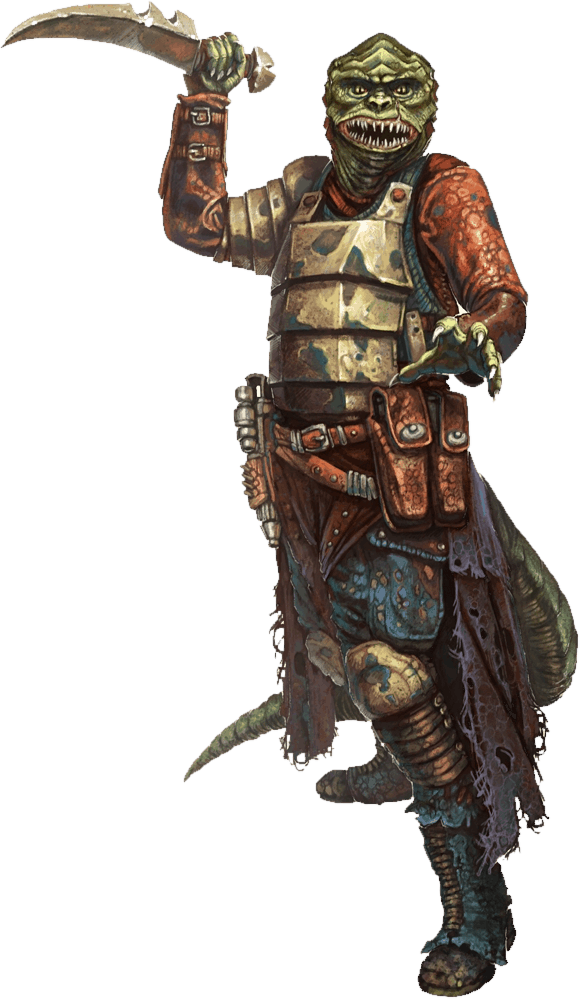
\includegraphics[width=5cm]{img/races/barabel.png}}
	\hline
	\basics[%
		type = Reptile,
		planet = Barab I,
		language = Barabel
	]
	\hline
	\traits
	\stats
	\hline
	Originaire de Barab I, les Barabels sont resté une race relativement primitive et isolée. Les Barabels vivent en clans dans un société principalement matriarcale. Ils sont fasciné par la guerre, la violence et les armes. Les Barabels ne sont pas profondément cruels mais il restent agressif de nature. En raison des nombreux rituels précédent les négociations, la diplomatie avec les Barabels est un exercice compliqué.
\end{monsterbox}

\begin{monsterbox}{Bothan}
	\textit{Small metasyntatic variable (golbinoid), neutral evil}\\
	\hline
	\basics[%
	type = Félin,
	planet = Bothawui,
	language = Bothese
	]
	\hline
	\traits[
    AGI = \stat{8} % This stat command will autocomplete the modifier for you
	]
	\stats[
    RES = 0 % This stat command will autocomplete the modifier for you
	]

	\hline
	
	\details[%
	% If you want to use commas in these sections, enclose the description in braces.
	size = 1m50
	]
	\hline 
	\monstersection{Descriptif}
	Les Bothans sont des humanoïdes trappus, dont le corps est recouvert d'une épaisse fourrure, donc les ondulations sont directement le reflet des sentiments éprouvés par ces êtres. 
  	Le peuple bothan est originaire de la planète Bothawui, un monde cosmopolite épargné des troubles de la Guerre Civile Galactique en raison de la neutralité officielle du gouvernement bothan. Plusieurs colonies ont également été construites sur des planètes proches, telles que Kothlis, qui est désormais le siège d'une importante communauté. Toutes ces colonies forment l'Espace Bothan. 
	\monstersection{Actions}
	\begin{monsteraction}[Generate text]
		This one can generate tremendous amounts of text! Though only when it wants to.
	\end{monsteraction}

	\begin{monsteraction}[More actions]
    See, here he goes again! Yet more text.
	\end{monsteraction}
\end{monsterbox}

\begin{quotebox}
	As you approach this template you get a sense that the blood and tears of many generations went into its making. A warm feeling welcomes you as you type your first words.
\end{quotebox}

\newpage % Acts as columbreak because of twocolumn option; for pagebreak use \clearpage

% For more columns, you can say \begin{dndtable}[your options here}.
% For instance, if you wanted three columns, you could say
% \begin{dndtable}{XXX}. The usual host of tabular parameters are
% aailable as well.
\header{Nice table}
\begin{dndtable}
   	\textbf{Table head}  & \textbf{Table head} \\
   	Some value  & Some value \\
   	Some value  & Some value \\
   	Some value  & Some value
\end{dndtable}

\begin{paperbox}{Do the Players need direction?}
	\lipsum[1]
\end{paperbox}

% You can optionally not include the background by saying
% begin{monsterboxnobg}
% \begin{monsterbox}{Monster Foo}
% 	\textit{Small metasyntatic variable (golbinoid), neutral evil}\\
% 	\hline
% 	\basics[%
% 	armorclass = 12,
% 	hitpoints  = 16 (3d8 + 3),
% 	speed      = 50 ft
% 	]
% 	\hline
% 	\stats[
%     STR = \stat{12}, % This stat command will autocomplete the modifier for you
%     DEX = \stat{7}
% 	]
% 	\hline
% 	\details[%
% 	% If you want to use commas in these sections, enclose the
% 	% description in braces.
% 	% I'm so sorry.
% 	languages = {Common Lisp, Erlang},
% 	]
% 	\hline \\[1mm]
% 	\begin{monsteraction}[Monster-super-powers]
% 		This Monster has some serious superpowers!
% 	\end{monsteraction}
% 	\monstersection{Actions}
% 	\begin{monsteraction}[Generate text]
% 		This one can generate tremendous amounts of text! Though only when it wants to.
% 	\end{monsteraction}
% 
% 	\begin{monsteraction}[More actions]
%     See, here he goes again! Yet more text.
% 	\end{monsteraction}
% \end{monsterbox}
